%!TeX root=../houndtop.tex
\chapter{The Man on the Tor}
\lettrine[lines=1]{T}{he} extract from my private diary which forms the last chap\-ter has brought my narrative up to the 18\textsuperscript{th} of October, a time when these strange events began to move swiftly towards their terrible conclusion. The incidents of the next few days are indelibly graven upon my recollection, and I can tell them without reference to the notes made at the time. I start then from the day which succeeded that upon which I had established two facts of great importance, the one that Mrs Laura Lyons of Coombe Tracey had written to Sir Charles Baskerville and made an appointment with him at the very place and hour that he met his death, the other that the lurking man upon the moor was to be found among the stone huts upon the hill-side. With these two facts in my possession I felt that either my intelligence or my courage must be deficient if I could not throw some further light upon these dark places.

I had no opportunity to tell the baronet what I had learned about Mrs Lyons upon the evening before, for Dr Mortimer remained with him at cards until it was very late. At breakfast, however, I informed him about my discovery, and asked him whether he would care to accompany me to Coombe Tracey. At first he was very eager to come, but on second thoughts it seemed to both of us that if I went alone the results might be better. The more formal we made the visit the less information we might obtain. I left Sir Henry behind, therefore, not without some prickings of conscience, and drove off upon my new quest.

When I reached Coombe Tracey I told Perkins to put up the horses, and I made inquiries for the lady whom I had come to interrogate. I had no difficulty in finding her rooms, which were central and well appointed. A maid showed me in without ceremony, and as I entered the sitting-room a lady, who was sitting before a Remington typewriter, sprang up with a pleasant smile of welcome. Her face fell, however, when she saw that I was a stranger, and she sat down again and asked me the object of my visit.

The first impression left by Mrs Lyons was one of extreme beau\-ty. Her eyes and hair were of the same rich hazel colour, and her cheeks, though considerably freckled, were flushed with the exquisite bloom of the brunette, the dainty pink which lurks at the heart of the sulphur rose. Admiration was, I repeat, the first impression. But the second was criticism. There was something subtly wrong with the face, some coarseness of expression, some hardness, perhaps, of eye, some looseness of lip which marred its perfect beauty. But these, of course, are after-thoughts. At the moment I was simply conscious that I was in the presence of a very handsome woman, and that she was asking me the reasons for my visit. I had not quite understood until that instant how delicate my mission was.

»I have the pleasure,« said I, »of knowing your father.« It was a clumsy introduction, and the lady made me feel it.

\begin{figure}[tbph]
\centering

\includegraphics[width=\linewidth]{10_extraordinary}
\caption{»Really, sir, this is a very extraordinary question.«}
\end{figure}

»There is nothing in common between my father and me,« she said. »I owe him nothing, and his friends are not mine. If it were not for the late Sir Charles Baskerville and some other kind hearts I might have starved for all that my father cared.«

»It was about the late Sir Charles Baskerville that I have come here to see you.«

The freckles started out on the lady's face.

»What can I tell you about him?« she asked, and her fingers played nervously over the stops of her typewriter.

»You knew him, did you not?«

»I have already said that I owe a great deal to his kindness. If I am able to support myself it is largely due to the interest which he took in my unhappy situation.«

»Did you correspond with him?«

The lady looked quickly up with an angry gleam in her hazel eyes.

»What is the object of these questions?« she asked sharply.

»The object is to avoid a public scandal. It is better that I should ask them here than that the matter should pass outside our control.«

She was silent and her face was still very pale. At last she looked up with something reckless and defiant in her manner.

»Well, I'll answer,« she said. »What are your questions?«

»Did you correspond with Sir Charles?«

»I certainly wrote to him once or twice to acknowledge his delicacy and his generosity.«

»Have you the dates of those letters?«

»No.«

»Have you ever met him?«

»Yes, once or twice, when he came into Coombe Tracey. He was a very retiring man, and he preferred to do good by stealth.«

»But if you saw him so seldom and wrote so seldom, how did he know enough about your affairs to be able to help you, as you say that he has done?«

She met my difficulty with the utmost readiness.

»There were several gentlemen who knew my sad history and united to help me. One was Mr Stapleton, a neighbour and intimate friend of Sir Charles's. He was exceedingly kind, and it was through him that Sir Charles learned about my affairs.«

I knew already that Sir Charles Baskerville had made Stapleton his almoner upon several occasions, so the lady's statement bore the impress of truth upon it.

»Did you ever write to Sir Charles asking him to meet you?« I continued.

Mrs Lyons flushed with anger again.

»Really, sir, this is a very extraordinary question.«

»I am sorry, madam, but I must repeat it.«

»Then I answer, certainly not.«

»Not on the very day of Sir Charles's death?«

The flush had faded in an instant, and a deathly face was before me. Her dry lips could not speak the »No« which I saw rather than heard.

»Surely your memory deceives you,« said I. »I could even quote a passage of your letter. It ran »Please, please, as you are a gentleman, burn this letter, and be at the gate by ten o'clock.««

I thought that she had fainted, but she recovered herself by a supreme effort.

»Is there no such thing as a gentleman?« she gasped.

»You do Sir Charles an injustice. He \emph{did} burn the letter. But sometimes a letter may be legible even when burned. You acknowledge now that you wrote it?«

»Yes, I did write it,« she cried, pouring out her soul in a torrent of words. »I did write it. Why should I deny it? I have no reason to be ashamed of it. I wished him to help me. I believed that if I had an interview I could gain his help, so I asked him to meet me.«

»But why at such an hour?«

»Because I had only just learned that he was going to London next day and might be away for months. There were reasons why I could not get there earlier.«

»But why a rendezvous in the garden instead of a visit to the house?«

»Do you think a woman could go alone at that hour to a bachelor's house?«

»Well, what happened when you did get there?«

»I never went.«

»Mrs Lyons!«

»No, I swear it to you on all I hold sacred. I never went. Something intervened to prevent my going.«

»What was that?«

»That is a private matter. I cannot tell it.«

»You acknowledge then that you made an appointment with Sir Charles at the very hour and place at which he met his death, but you deny that you kept the appointment.«

»That is the truth.«

Again and again I cross-questioned her, but I could never get past that point.

»Mrs Lyons,« said I, as I rose from this long and inconclusive interview, »you are taking a very great responsibility and putting yourself in a very false position by not making an absolutely clean breast of all that you know. If I have to call in the aid of the police you will find how seriously you are compromised. If your position is innocent, why did you in the first instance deny having written to Sir Charles upon that date?«

»Because I feared that some false conclusion might be drawn from it and that I might find myself involved in a scandal.«

»And why were you so pressing that Sir Charles should destroy your letter?«

»If you have read the letter you will know.«

»I did not say that I had read all the letter.«

»You quoted some of it.«

»I quoted the postscript. The letter had, as I said, been burned and it was not all legible. I ask you once again why it was that you were so pressing that Sir Charles should destroy this letter which he received on the day of his death.«

»The matter is a very private one.«

»The more reason why you should avoid a public investigation.«

»I will tell you, then. If you have heard anything of my unhappy history you will know that I made a rash marriage and had reason to regret it.«

»I have heard so much.«

»My life has been one incessant persecution from a husband whom I abhor. The law is upon his side, and every day I am faced by the possibility that he may force me to live with him. At the time that I wrote this letter to Sir Charles I had learned that there was a prospect of my regaining my freedom if certain expenses could be met. It meant everything to me\allowbreak---\allowbreak peace of mind, happiness, self-respect\allowbreak---\allowbreak everything. I knew Sir Charles's generosity, and I thought that if he heard the story from my own lips he would help me.«

»Then how is it that you did not go?«

»Because I received help in the interval from another source.«

»Why then, did you not write to Sir Charles and explain this?«

»So I should have done had I not seen his death in the paper next morning.«

The woman's story hung coherently together, and all my questions were unable to shake it. I could only check it by finding if she had, indeed, instituted divorce proceedings against her husband at or about the time of the tragedy.

It was unlikely that she would dare to say that she had not been to Baskerville Hall if she really had been, for a trap would be necessary to take her there, and could not have returned to Coombe Tracey until the early hours of the morning. Such an excursion could not be kept secret. The probability was, therefore, that she was telling the truth, or, at least, a part of the truth. I came away baffled and disheartened. Once again I had reached that dead wall which seemed to be built across every path by which I tried to get at the object of my mission. And yet the more I thought of the lady's face and of her manner the more I felt that something was being held back from me. Why should she turn so pale? Why should she fight against every admission until it was forced from her? Why should she have been so reticent at the time of the tragedy? Surely the explanation of all this could not be as innocent as she would have me believe. For the moment I could proceed no farther in that direction, but must turn back to that other clue which was to be sought for among the stone huts upon the moor.

And that was a most vague direction. I realized it as I drove back and noted how hill after hill showed traces of the ancient people. Barrymore's only indication had been that the stranger lived in one of these abandoned huts, and many hundreds of them are scattered throughout the length and breadth of the moor. But I had my own experience for a guide since it had shown me the man himself standing upon the summit of the Black Tor. That then should be the centre of my search. From there I should explore every hut upon the moor until I lighted upon the right one. If this man were inside it I should find out from his own lips, at the point of my revolver if necessary, who he was and why he had dogged us so long. He might slip away from us in the crowd of Regent Street, but it would puzzle him to do so upon the lonely moor. On the other hand, if I should find the hut and its tenant should not be within it I must remain there, however long the vigil, until he returned. Holmes had missed him in London. It would indeed be a triumph for me if I could run him to earth, where my master had failed.

Luck had been against us again and again in this inquiry, but now at last it came to my aid. And the messenger of good fortune was none other than Mr Frankland, who was standing, gray-whiskered and red-faced, outside the gate of his garden, which opened on to the high road along which I travelled.

»Good-day, Dr Watson,« cried he with unwonted good hum\-our, »you must really give your horses a rest, and come in to have a glass of wine and to congratulate me.«

My feelings towards him were very far from being friendly after what I had heard of his treatment of his daughter, but I was anxious to send Perkins and the wagonette home, and the opportunity was a good one. I alighted and sent a message to Sir Henry that I should walk over in time for dinner. Then I followed Frankland into his dining-room.

\begin{figure}[tbh]
\centering

\includegraphics[width=.6\linewidth]{11_goodday}
\caption{»Good-day, Dr Watson,« cried he}
\end{figure}

»It is a great day for me, sir\allowbreak---\allowbreak one of the red-letter days of my life,« he cried with many chuckles. »I have brought off a double event. I mean to teach them in these parts that law is law, and that there is a man here who does not fear to invoke it. I have established a right of way through the centre of old Middleton's park, slap across it, sir, within a hundred yards of his own front door. What do you think of that? We'll teach these magnates that they cannot ride roughshod over the rights of the commoners, confound them! And I've closed the wood where the Fernworthy folk used to picnic. These infernal people seem to think that there are no rights of property, and that they can swarm where they like with their papers and their bottles. Both cases decided, Dr Watson, and both in my favour. I haven't had such a day since I had Sir John Morland for trespass, because he shot in his own warren.«

»How on earth did you do that?«

»Look it up in the books, sir. It will repay reading\allowbreak---\allowbreak Frankland \textit{v.} Morland, Court of Queen's Bench. It cost me \textsterling 200, but I got my verdict.«

»Did it do you any good?«

»None, sir, none. I am proud to say that I had no interest in the matter. I act entirely from a sense of public duty. I have no doubt, for example, that the Fernworthy people will burn me in effigy to-night. I told the police last time they did it that they should stop these disgraceful exhibitions. The County Constabulary is in a scandalous state, sir, and it has not afforded me the protection to which I am entitled. The case of Frankland \textit{v.} Regina will bring the matter before the attention of the public. I told them that they would have occasion to regret their treatment of me, and already my words have come true.«

»How so?« I asked.

The old man put on a very knowing expression.

»Because I could tell them what they are dying to know; but nothing would induce me to help the rascals in any way.«

I had been casting round for some excuse by which I could get away from his gossip, but now I began to wish to hear more of it. I had seen enough of the contrary nature of the old sinner to understand that any strong sign of interest would be the surest way to stop his confidences.

»Some poaching case, no doubt?« said I, with an indifferent manner.

»Ha, ha, my boy, a very much more important matter than that! What about the convict on the moor?«

I started. »You don't mean that you know where he is?« said I.

»I may not know exactly where he is, but I am quite sure that I could help the police to lay their hands on him. Has it never struck you that the way to catch that man was to find out where he got his food, and so trace it to him?«

He certainly seemed to be getting uncomfortably near the truth. »No doubt,« said I; »but how do you know that he is anywhere upon the moor?«

»I know it because I have seen with my own eyes the messenger who takes him his food.«

My heart sank for Barrymore. It was a serious thing to be in the power of this spiteful old busybody. But his next remark took a weight from my mind.

»You'll be surprised to hear that his food is taken to him by a child. I see him every day through my telescope upon the roof. He passes along the same path at the same hour, and to whom should he be going except to the convict?«

Here was luck indeed! And yet I suppressed all appearance of interest. A child! Barrymore had said that our unknown was supplied by a boy. It was on his track, and not upon the convict's, that Frankland had stumbled. If I could get his knowledge it might save me a long and weary hunt. But incredulity and indifference were evidently my strongest cards.

»I should say that it was much more likely that it was the son of one of the moorland shepherds taking out his father's dinner.«

The least appearance of opposition struck fire out of the old autocrat. His eyes looked malignantly at me, and his gray whiskers bristled like those of an angry cat.

»Indeed, sir!« said he, pointing out over the wide-stretching moor. »Do you see that Black Tor over yonder? Well, do you see the low hill beyond with the thornbush upon it? It is the stoniest part of the whole moor. Is that a place where a shepherd would be likely to take his station? Your suggestion, sir, is a most absurd one.«

I meekly answered that I had spoken without knowing all the facts. My submission pleased him and led him to further confidences.

»You may be sure, sir, that I have very good grounds before I come to an opinion. I have seen the boy again and again with his bundle. Every day, and sometimes twice a day, I have been able\allowbreak---\allowbreak but wait a moment, Dr Watson. Do my eyes deceive me, or is there at the present moment something moving upon that hill- side?«

It was several miles off, but I could distinctly see a small dark dot against the dull green and gray.

»Come, sir, come!« cried Frankland, rushing upstairs. »You will see with your own eyes and judge for yourself.«

The telescope, a formidable instrument mounted upon a tripod, stood upon the flat leads of the house. Frankland clapped his eye to it and gave a cry of satisfaction.

»Quick, Dr Watson, quick, before he passes over the hill!«

There he was, sure enough, a small urchin with a little bundle upon his shoulder, toiling slowly up the hill. When he reached the crest I saw the ragged uncouth figure outlined for an instant against the cold blue sky. He looked round him with a furtive and stealthy air, as one who dreads pursuit. Then he vanished over the hill.

»Well! Am I right?«

»Certainly, there is a boy who seems to have some secret errand.«

»And what the errand is even a county constable could guess. But not one word shall they have from me, and I bind you to secrecy also, Dr Watson. Not a word! You understand!«

»Just as you wish.«

»They have treated me shamefully\allowbreak---\allowbreak shamefully. When the facts come out in Frankland \textit{v.} Regina I venture to think that a thrill of indignation will run through the country. Nothing would induce me to help the police in any way. For all they cared it might have been me, instead of my effigy, which these rascals burned at the stake. Surely you are not going! You will help me to empty the decanter in honour of this great occasion!«

But I resisted all his solicitations and succeeded in dissuading him from his announced intention of walking home with me. I kept the road as long as his eye was on me, and then I struck off across the moor and made for the stony hill over which the boy had disappeared. Everything was working in my favour, and I swore that it should not be through lack of energy or perseverance that I should miss the chance which fortune had thrown in my way.

\begin{figure}[tbh]
\centering

\includegraphics[width=.7\linewidth]{11_frankscope}
\caption{Frankland clapped his eye to it and gave a cry of satisfaction.}
\end{figure}

The sun was already sinking when I reached the summit of the hill, and the long slopes beneath me were all golden-green on one side and gray shadow on the other. A haze lay low upon the farthest sky-line, out of which jutted the fantastic shapes of Belliver and Vixen Tor. Over the wide expanse there was no sound and no movement. One great gray bird, a gull or curlew, soared aloft in the blue heaven. He and I seemed to be the only living things between the huge arch of the sky and the desert beneath it. The barren scene, the sense of loneliness, and the mystery and urgency of my task all struck a chill into my heart. The boy was nowhere to be seen. But down beneath me in a cleft of the hills there was a circle of the old stone huts, and in the middle of them there was one which retained sufficient roof to act as a screen against the weather. My heart leaped within me as I saw it. This must be the burrow where the stranger lurked. At last my foot was on the threshold of his hiding place\allowbreak---\allowbreak his secret was within my grasp.

As I approached the hut, walking as warily as Stapleton would do when with poised net he drew near the settled butterfly, I satisfied myself that the place had indeed been used as a habitation. A vague pathway among the boulders led to the dilapidated opening which served as a door. All was silent within. The unknown might be lurking there, or he might be prowling on the moor. My nerves tingled with the sense of adventure. Throwing aside my cigarette, I closed my hand upon the butt of my revolver and, walking swiftly up to the door, I looked in. The place was empty.

But there were ample signs that I had not come upon a false scent. This was certainly where the man lived. Some blankets rolled in a waterproof lay upon that very stone slab upon which Neolithic man had once slumbered. The ashes of a fire were heaped in a rude grate. Beside it lay some cooking utensils and a bucket half-full of water. A litter of empty tins showed that the place had been occupied for some time, and I saw, as my eyes became accustomed to the chequered light, a pannikin and a half-full bottle of spirits standing in the corner. In the middle of the hut a flat stone served the purpose of a table, and upon this stood a small cloth bundle\allowbreak---\allowbreak the same, no doubt, which I had seen through the telescope upon the shoulder of the boy. It contained a loaf of bread, a tinned tongue, and two tins of preserved peaches. As I set it down again, after having examined it, my heart leaped to see that beneath it there lay a sheet of paper with writing upon it. I raised it, and this was what I read, roughly scrawled in pencil:\allowbreak---\allowbreak  

\begin{figure}[p]
\centering
\includegraphics[width=\linewidth]{12_shadow}
\caption{A shadow fell across the opening of the hut.}
\end{figure}

\textit{Dr Watson has gone to Coombe Tracey.}

For a minute I stood there with the paper in my hands thinking out the meaning of this curt message. It was I, then, and not Sir Henry, who was being dogged by this secret man. He had not followed me himself, but he had set an agent\allowbreak---\allowbreak the boy, perhaps\allowbreak---\allowbreak upon my track, and this was his report. Possibly I had taken no step since I had been upon the moor which had not been observed and reported. Always there was this feeling of an unseen force, a fine net drawn round us with infinite skill and delicacy, holding us so lightly that it was only at some supreme moment that one realized that one was indeed entangled in its meshes.

If there was one report there might be others, so I looked round the hut in search of them. There was no trace, however, of anything of the kind, nor could I discover any sign which might indicate the character or intentions of the man who lived in this singular place, save that he must be of Spartan habits and cared little for the comforts of life. When I thought of the heavy rains and looked at the gaping roof I understood how strong and immutable must be the purpose which had kept him in that inhospitable abode. Was he our malignant enemy, or was he by chance our guardian angel? I swore that I would not leave the hut until I knew.

Outside the sun was sinking low and the west was blazing with scarlet and gold. Its reflection was shot back in ruddy patches by the distant pools which lay amid the great Grimpen Mire. There were the two towers of Baskerville Hall, and there a distant blur of smoke which marked the village of Grimpen. Between the two, behind the hill, was the house of the Stapletons. All was sweet and mellow and peaceful in the golden evening light, and yet as I looked at them my soul shared none of the peace of nature but quivered at the vagueness and the terror of that interview which every instant was bringing nearer. With tingling nerves, but a fixed purpose, I sat in the dark recess of the hut and waited with sombre patience for the coming of its tenant.

And then at last I heard him. Far away came the sharp clink of a boot striking upon a stone. Then another and yet another, coming nearer and nearer. I shrank back into the darkest corner, and cocked the pistol in my pocket, determined not to discover myself until I had an opportunity of seeing something of the stranger. There was a long pause which showed that he had stopped. Then once more the footsteps approached and a shadow fell across the opening of the hut.

»It is a lovely evening, my dear Watson,« said a well-known voice. »I really think that you will be more comfortable outside than in.«

\clearpage
\newpage
\vfill
\begin{figure}[tbph]
\centering
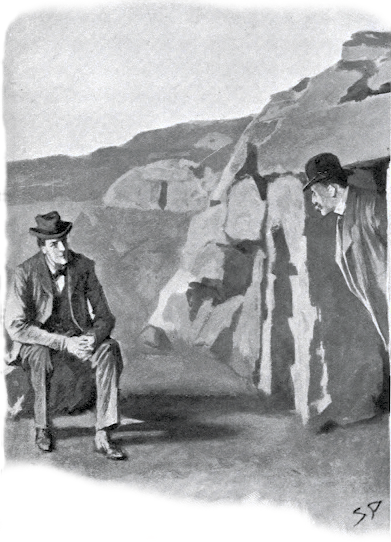
\includegraphics[width=\linewidth]{12_therehesat}
\caption{There he sat upon a stone}
\end{figure}
\vfill
\thispagestyle{empty}
\clearpage